%! TEX TS-program = lualatex
%! TeX root = doc/slides.tex

\documentclass[aspectratio=169]{beamer}

\newcommand{\names}{Gabriel \textsc{Doriath Döhler}, Constantin \textsc{Gierczak--Galle}}

\title{"Craft your IC"\\Learning hardware design in
Minecraft\footnote{\tiny{}\reproduce}\\\small{} École Normale Supérieure, Paris (ENS Ulm)}
\author{\names}
\institute{FSiC $2023$}
\date{July $12$, $2023$}

\usepackage{fontspec}
\setmonofont{FreeMono}
\usepackage{amsmath}
\usepackage{listings}
\usepackage{xcolor}
\usepackage{qrcode}
\usepackage{caption}

\newcommand{\rv}{\texttt{RISC-V}}
\newcommand{\vrv}{\texttt{V-\rv}}
\newcommand{\hw}{HW}
% FIXME: Update this with the new link
% Also, add a clickable link for the handouts
\newcommand{\rvlink}{https://github.com/gabriel-doriath-dohler/Craft-your-IC}

\setcounter{tocdepth}{1}

\begin{document}
\beamertemplatenavigationsymbolsempty
\addtobeamertemplate{navigation symbols}{}{%
	\usebeamerfont{footline}%
	\usebeamercolor[fg]{footline}%
	\hspace{1em}%
	\insertframenumber/\inserttotalframenumber
}

\maketitle

\begin{frame}[fragile]
	\frametitle{Story time}
	\begin{figure}
		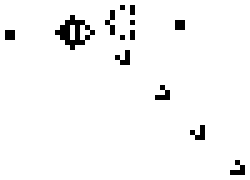
\includegraphics[width=.5\textwidth]{imgs/game_of_life.png}
		\caption*{Conway's game of life, by Lucas Vieira - Own work, CC BY-SA 3.0, https://commons.wikimedia.org/w/index.php?curid=101736}
	\end{figure}

	% game of life turing machine
	% borrow computational construct from the game
	% sysnum CPU, cst1 + gdd idée MC
	% but there is one problem: know that we had the idea, we had to do it, somehow the TAs accepted
	% but why???
	% - Minecraft is a good interactive tool to learn hardware concepts
	% - BUT IT'S ALSO VERY FUN
\end{frame}

\begin{frame}[fragile]
	\frametitle{Table of Contents}
	\tableofcontents
\end{frame}

\section{Logic circuits in Minecraft (gdd)}

 {
  \usebackgroundtemplate{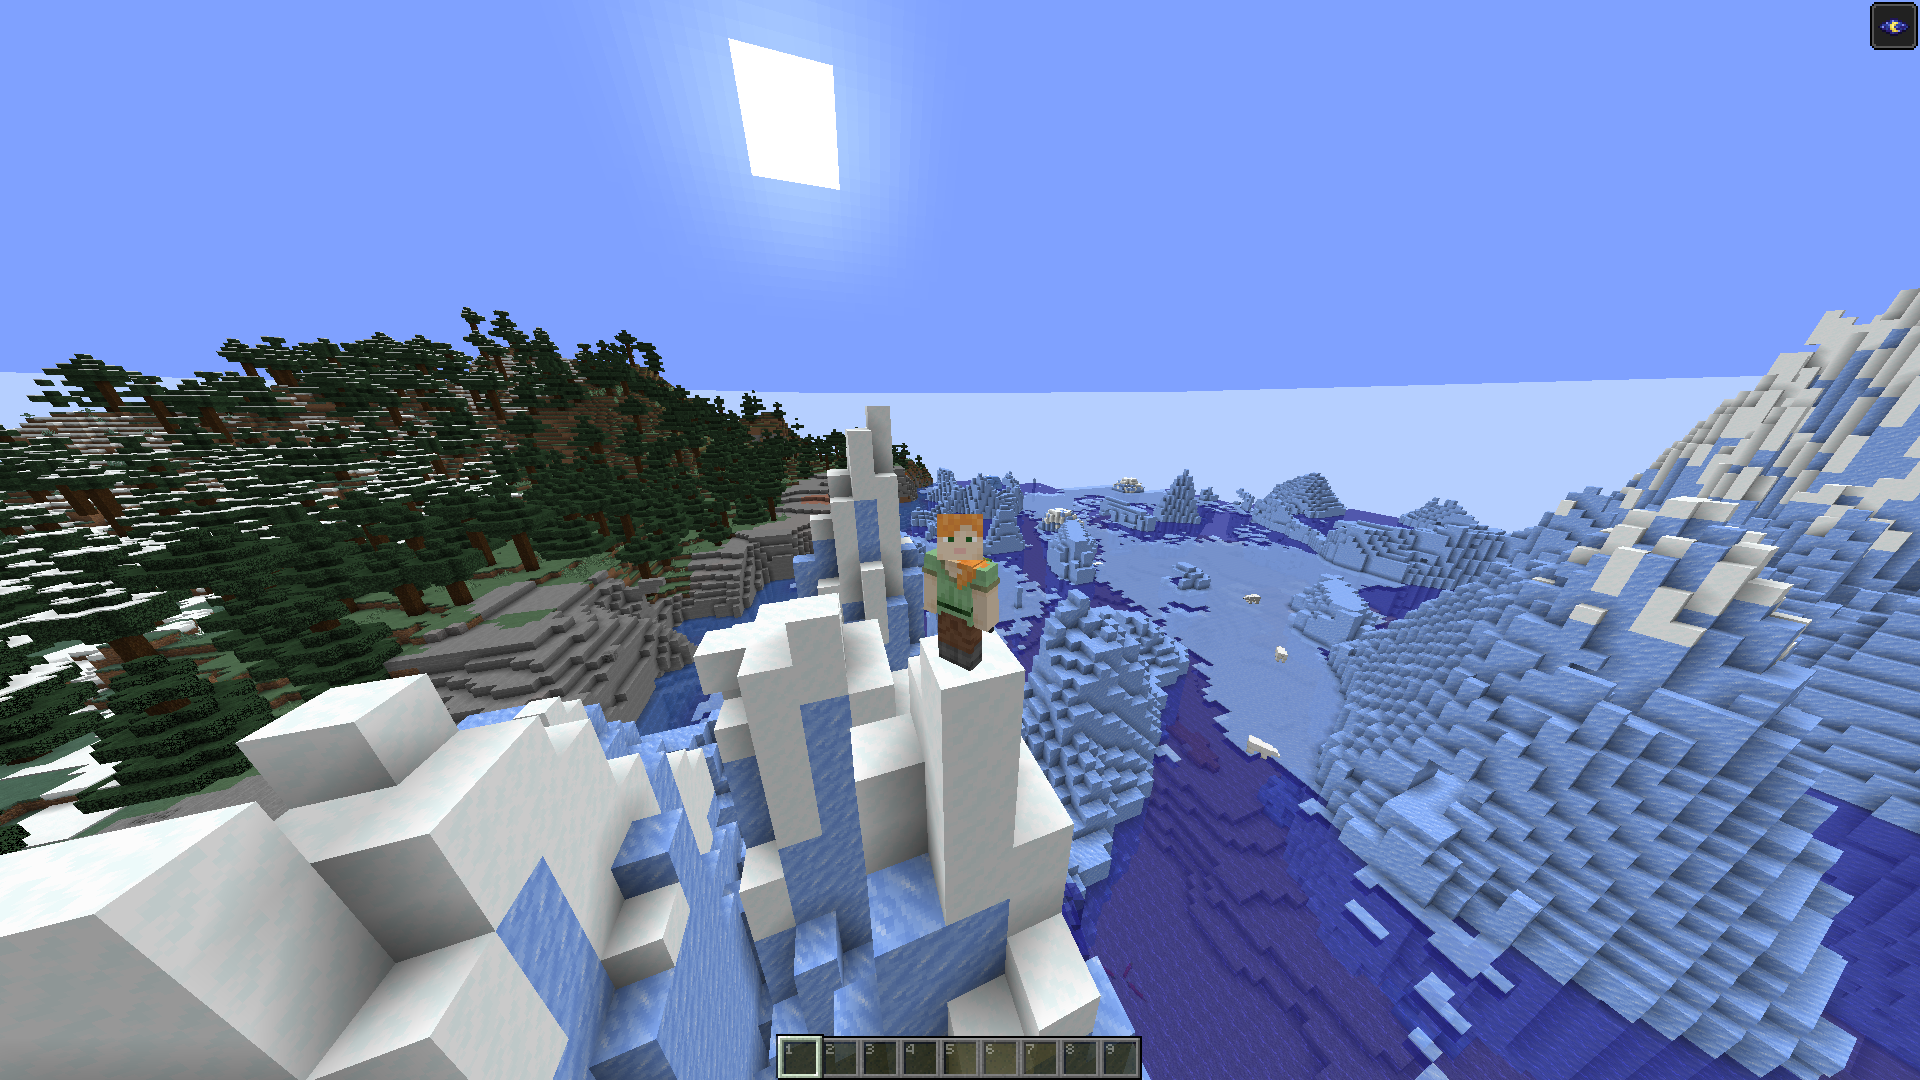
\includegraphics[width=\paperwidth]{imgs/minecraft.png}}
  \begin{frame}[plain]
	  % block game owned by microsoft (not open source but reverse friendly)
	  % a player moves and can place/delete cubes (called blocks) in a grid
  \end{frame}
 }

\begin{frame}
	\frametitle{Minecraft Redstone}

	\begin{columns}
		\begin{column}{0.5\textwidth}
			Redstone = equivalent of electronics
			\begin{itemize}
				\item<1->{Lever = player input}
				\item<1->{Lamp = output}

				\item<2->{Redstone = wires}

				\item<3->{Torch = NOT gate}
				\item<3->{1 tick = 0.1 sec}

				\item<4->{Repeater}
				\begin{itemize}
					\item<4->{delay element}
					\item<4->{diode}
					\item<4->{amplifier}
					\item<4->{memory cell}
				\end{itemize}

				\item<4->{Many more redstone components...}
			\end{itemize}
		\end{column}
		\begin{column}{0.5\textwidth}
			\begin{center}
				\includegraphics<1>[width=0.9\textwidth]{imgs/lamp.png}

				\includegraphics<2>[width=0.4\textwidth]{imgs/wire.png}
				\includegraphics<2>[width=0.4\textwidth]{imgs/or_gate.png}
				\includegraphics<2>[width=0.4\textwidth]{imgs/fanout.png}

				\includegraphics<3>[width=0.7\textwidth]{imgs/torch_on.png}
				\includegraphics<3>[width=0.7\textwidth]{imgs/torch_off.png}

				\includegraphics<4>[width=0.4\textwidth]{imgs/repeater_delay_off.png}
				\includegraphics<4>[width=0.4\textwidth]{imgs/repeater_delay_on.png}
				\includegraphics<4>[width=0.5\textwidth]{imgs/repeater_diode.png}

				\includegraphics<5>[width=0.9\textwidth]{imgs/repeater_clock.png}

				\includegraphics<6>[height=0.8\textheight]{imgs/power_strength.png}
				\includegraphics<6>[height=0.8\textheight]{imgs/repeater_amplifier.png}

				\includegraphics<7>[width=0.9\textwidth]{imgs/repeater_memory_cell.png}
			\end{center}
		\end{column}
	\end{columns}

	% can't have 4 meters of cables like in tiny tapeout

\end{frame}

\begin{frame}
	\frametitle{Minecraft Redstone: unusual behavior}

	\begin{columns}
		\begin{column}{0.5\textwidth}
			\begin{itemize}
				\item<1->Comparators =\\ weird transistors with 2 modes:
				\begin{itemize}
					\item<1->{Compare mode transmits iff\\ main input $\geq$ side input}
					\item<1->{Substract =\\ max(0, main input - side input)}
				\end{itemize}
				\item<2->{Slab = instant diode}
			\end{itemize}
		\end{column}
		\begin{column}{0.5\textwidth}
			\begin{center}
				\includegraphics<1>[width=0.7\textwidth]{imgs/cmp.png}
				\includegraphics<1>[width=0.7\textwidth]{imgs/cmp_sub.png}

				\includegraphics<2>[width=0.9\textwidth]{imgs/slab.png}
			\end{center}
		\end{column}
	\end{columns}
	% skip barrels

	MC = netlist simulator for 4-bit valued signals
\end{frame}

\begin{frame}
	\frametitle{Building Circuits!}
	we already built a clock and a memory cell
	example of simple circuits
	half adder (in game)
	MUX/DEMUX?
	cool minecraft tech: CCA adder (Yap7 + Magic:\^ (2014)))
	$$cc_i = carry_cancel_i = cancel_i = a_i nand b_i = not propagate$$
	$$g_i = generate_i = a_1 and b_i$$
	$$c_{i+1} = (not cancel_i) and (generate_i or ((not cancel_{i-1}) and (generate_{i-1} or ...)))$$
	$$= ((not cancel_i) and generate_i) or ((not cancel_i) and (not cancel_{i-1}) and generate_{i-1}) or ...$$
	$$= sum_{j=0}^{i} generate_{j} and prod_{k=j}^{i} ¬cancel_k$$
	$$slabTower_{g_i} = max power strength_{j=0}^{i-1} generate_j$$
	$$slabTower_{cc_i} = max power strength_{j=0}^{i-1} cc_j$$
	works because a carry that is later canceled will have less power strength on th towers
	$$c_{i+1} = slabTower_{g_i} > slabTower_{cc_i}$$
	$$c_0 = carry_in$$
	$$a_n = b_n = 0$$
	$$o_i = a_i xor b_i xor c_i$$
	cancel doesn't have to be accurate (use NOR)

	7 ticks design (5 tick possible?)
	fully synchronized
	pipeline every 1 or 2 ticks
\end{frame}

\begin{frame}
	\frametitle{Minecraft vs "Real" Hardware: what's different?}
	power strength
	instant diodes
	no tooling: HDL, version control, GTKWave, test framework
	the physical layer is much more constraining: wires are big and connect automatically, but being compact is necessary for performance
\end{frame}

\section{"Craft your IC" Design and ISA (cst1)}

% note for cst1: i would talk about:
% - ISA choice (why not RISV-V?)
% - debuging (replay mod)
% - wirering the different parts is a challenge
% - decoding instruction is trivial because of instruction length
% - simple pipeline (wave pipeline) (not done yet)
% - the things you already mention

\begin{frame}
	\frametitle{Instruction Set Architecture}
	%\vrv
	%\texttt{(Very-RISC)-V}

	$8$-bit registers:

	\begin{itemize}
		\item \texttt{\%0}: $00000000$ -- like \rv{}
		\item \texttt{\%1}: $11111111$ -- for $1$--op \texttt{inc}
		      \texttt{dec}, \texttt{not}
		\item \texttt{\%2}-\texttt{\%14}: GP registers
		\item \texttt{\%15}: Random register
	\end{itemize}

	\pause

	Instructions:
	\begin{itemize}
		\item \textbf{Binops}: \texttt{add}, \texttt{sub}, \texttt{or},
		      \texttt{xor}: $3$ register operands
		\item \textbf{Jumps}: unconditional or on
		      \texttt{oveflow}/\texttt{negative}/\texttt{zero}
		\item \texttt{loadi}: Load immediate to register
		\item \textbf{RAM}: Load and store
		\item \texttt{print}: prints a byte to a 7-segment display
	\end{itemize}
\end{frame}

\subsection{An $8$-bit CPU (???)}
% Harvard architecthture (separate ROM and RAM)
% 8 bits because max power strength is 15 so the ALU towers do not need repeaters
\begin{frame}
	Rapidly list all components

	For each component, make a 2-column slide, the left column contains some
	interesting bulletpoints, the right one a picture of said components (if
	possible isolated?)
\end{frame}

\begin{frame}
	\frametitle{ROM and PC}
	\begin{columns}
		\begin{column}{0.4\textwidth}
			\begin{itemize}
				\item $128$ instruction ROM
				\item Bits encoded as presence/absence of power blocks in a grid
			\end{itemize}
		\end{column}
		\begin{column}{0.6\textwidth}
			\begin{center}
				\includegraphics<1>[width=0.8\textwidth]{imgs/rom.png}
				\includegraphics<2->[width=0.325\textwidth]{imgs/pc.png}

				\framesubtitle<1>{ROM bank}
				\framesubtitle<2->{Program Counter}
			\end{center}
		\end{column}
	\end{columns}
\end{frame}

\begin{frame}
	\frametitle{Registers}
	\begin{columns}
		\begin{column}{0.5\textwidth}
			\begin{itemize}
				\item All registers doubled for double--read
				\item \texttt{\%0} and \texttt{\%1} hard-wired
				\item \texttt{\%15} random register uses Minecraft randomizers
			\end{itemize}
		\end{column}
		\begin{column}{0.5\textwidth}
			\begin{center}
				\includegraphics<1>[width=0.9\textwidth]{imgs/register_slice.png}
				\includegraphics<2->[width=0.9\textwidth]{imgs/register_file.png}

				\framesubtitle<1>{Register}
				\framesubtitle<2->{Register file}
			\end{center}
		\end{column}
	\end{columns}
\end{frame}

\begin{frame}
	\frametitle{ALU}
	\begin{columns}
		\begin{column}{0.4\textwidth}
			\begin{itemize}
				\item Combinatorial
				\item Compact design for speed.
			\end{itemize}
		\end{column}
		\begin{column}{0.6\textwidth}
			\begin{center}
				\includegraphics<1>[width=\textwidth]{imgs/alu_slice.png}
				\includegraphics<2->[width=0.8\textwidth]{imgs/alu.png}

				\framesubtitle<1>{ALU slice}
			\end{center}
		\end{column}
	\end{columns}
\end{frame}

\begin{frame}
	\frametitle{I/O}
	\begin{columns}
		\begin{column}{0.4\textwidth}
			\begin{itemize}
				\item \hw{} design in MC
				\item Formal verification
			\end{itemize}
		\end{column}
		\begin{column}{0.6\textwidth}
			\begin{figure}
				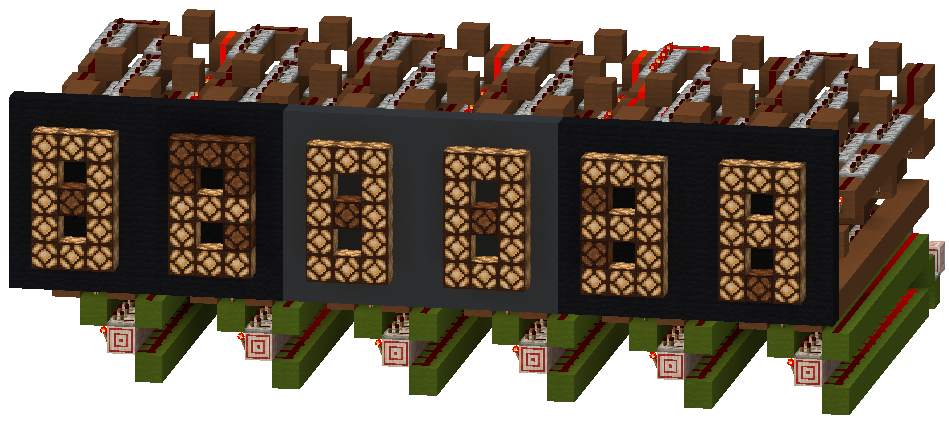
\includegraphics[width=\textwidth]{imgs/screen.png}
				\caption*{$7$-segment display}
			\end{figure}
		\end{column}
	\end{columns}
\end{frame}

\begin{frame}[fragile]
	\frametitle{Toolchain}
	\begin{columns}
		\begin{column}{0.4\textwidth}
			\begin{itemize}
				\item Assembler
			\end{itemize}
			\lstdefinelanguage{asm}
			{morekeywords={add, xor, jmp, jneg, loadi},
				sensitive=true,
				morecomment=[l]{--},
				morecomment=[s]{/*}{*/},
			}
			\lstset{language=asm}
			\begin{lstlisting}
.sec
	add %5 %2 %2
	xor %2 %1 %9
	add %5 %9 %9
	add %6 %9 %0
	jneg min
	jmp print_sec
.min
	loadi $0 %2
	add %5 %3 %3
	xor %3 %1 %9
	add %5 %9 %9
	add %6 %9 %0
	jneg hour
	jmp print_min
	\end{lstlisting}
		\end{column}
		\pause
		\begin{column}{0.6\textwidth}
			\begin{itemize}
				\item Linker
			\end{itemize}
			Resolves label references and computes jumps
			\lstset{language=asm}
			\begin{lstlisting}
add %5 %2 %2
xor %2 %1 %9
add %5 %9 %9
add %6 %9 %0
jneg 0x10
jmp 0x03
	\end{lstlisting}
			\pause
			\begin{itemize}
				\item ROM generator
			\end{itemize}
			\lstdefinelanguage{command}
			{morekeywords={setblock, torch, air},
				sensitive=true,
				morecomment=[l]{--},
				morecomment=[s]{/*}{*/},
			}
			\lstset{language=command}
			\begin{lstlisting}
setblock -272 197 -1402 torch
setblock -270 197 -1402 torch
setblock -268 197 -1402 air
        \end{lstlisting}
		\end{column}
	\end{columns}
\end{frame}

\section{Demo (cst1)}

\begin{frame}
	\frametitle{The Demo (finally!)}
	clock
	e approximation using RNG
	joke: very secure because: active temper detection with TNT + industry grade (aka. java) RNG.
\end{frame}

\section{The community (cst1)}

\begin{frame}
	\frametitle{The community}
	\framesubtitle{Other processors}

	https://openredstone.org/

	Talk about MineTest, as a possible OS replacement for MC.
\end{frame}

\begin{frame}
	\frametitle{The community}
	\framesubtitle{Open-source tools}

\end{frame}

\begin{frame}
	ORE
	Chungus 2
	minecraft in minecraft
	similar to traditional FOSS communities
	license
	they make sure to give credits to creators of designs

	toolchain:
	- prismlauncher and quilt mod loader
	- ressource pack vanilla tweaks
	- worldedit (copy paste)
	- replay mod (debugging and rendering)
	- carpet (tick rate control + noclip and more)
	- ferritecore, immediatelyFast, lithium, sodium (optimizations)
	- Xaero's World Map (waypoints)
	- Tweakeroo (flexible and accurate block placement)
	- litematica
	- isometric renders (renders)
	- MCHPRS (gdd?)

	Talk about the community doing crazy CPUs in MC, drop a picture, some
	links, etc.
\end{frame}

\section{Perspectives and Verification (gdd can skip if needed)}
\begin{frame}
	\frametitle{Perspectives}
	\begin{itemize}
		\item arm cortex A53
		\item RV32-I
		\item dynamic FPGA
		\item MCHPS
		\item semantics and formal verification
	\end{itemize}
\end{frame}

\begin{frame}
	\frametitle{Verifying HW semantics}
	MC semantics
	ALU graph
	haskell k induction
	results
	stats number of blocks (part's list)
	so way too big for SMT
	plan: use model checking with a lean DSL and state machines



	Notes: On n'a pas de HDL (expliquer pourquoi et donner le lien du HDL existant)
	Mentionner l'état de l'art (~inexistant) en génération de circuit MC à
	partir de HDL.

	Donc pour vérifier le CPU, on vérifie... Le CPU! Pas la source.
	Donc on raisonne directement sur le """silicium"""
\end{frame}

\section{Educational Aspects (gdd + cst1)}

\begin{frame}
	\frametitle{Learning Outcomes}
	testimonials from ORE who became "real" hardware people
	talent pool to recruit from
	MC is an interactive tool
	lecture at Harvard
	16 yo
	graphics rendering
	asm
	LLVM-like optimization stages for MCHPRS

	asm
	linker
	CPU design
	verification

	teaching redstone to my brother is simpler than verilog

	what we learned
\end{frame}

\begin{frame}
	\frametitle{Acknowledgement}
	\begin{columns}
		\begin{column}{0.5\textwidth}
			Special thanks to friends and collaborators on this projects,
			including:
			\begin{itemize}
				\item Hadrien Barral
				\item Rémy Citerin
			\end{itemize}
		\end{column}
		\begin{column}{0.5\textwidth}
			A big thank you to the FSiC committee for hosting our talk!
			\begin{figure}
				
\includegraphics[width=0.75\textwidth]{imgs/Fsic2023_logo.png}
			\end{figure}
		\end{column}
	\end{columns}
\end{frame}

\begin{frame}[fragile]
	\frametitle{Q/A}
	\begin{columns}
		\begin{column}{0.4\textwidth}
			% TODO Add key points of the talk
			\begin{itemize}
				\item \hw{} design in Minecraft
				\item ISA and implementation
				\item ASM-to-ROM toolchain
				\item Formal verification efforts
			\end{itemize}
		\end{column}
		\begin{column}{0.6\textwidth}
			\begin{center}
				Craft your IC project
				\\ \url{\rvlink}
				\begin{figure}
					\qrcode[height=4cm]{\rvlink}
				\end{figure}
			\end{center}
		\end{column}
	\end{columns}
	\begin{center}
		\small \names{}
	\end{center}
\end{frame}

\newpage
\bibliographystyle{plain}
\bibliography{ref}

\end{document}
